\chapter{Data-driven background estimation}\label{chap:bkgmodel}
This section outlines the procedure for the estimation of the background using the data-driven extrapolation approach. The procedure is motivated in chapter~\cref{sec:bkgmodel:motivation}. There are several challenges involved with the method. One challenge is the choice of function picked to model the fit in the low-mass CR and extrapolation to the high-mass SR. An optimisation procedure is performed in two consecutive steps. The first involves the choice of the fit function. An initial sample of 25 functions are validated in a set of potential CR and SR. The method used to chose the functional form is outlined in \cref{sec:modelchoice}. A signal+background function is defined in \cref{sec:sigmodel}, which is used to validate the CR and SR choice. Once the function is fixed, the CRs and SRs are optimised to maximise sensitivity and reduce the bias of the background estimation. The optimisation procedure is described in \cref{sec:extrap:optimisation}. All fits are performed within the RooFit~\cite{RooFit} framework.

\section{Motivation}\label{sec:bkgmodel:motivation}
The previous ATLAS search for non-resonant signals in the dilepton invariant-mass spectra was published with \SI{36.1}{\femto\barn^{-1}}~\cite{EXOT-2016-05}. The analysis used a MC template based approach to model the background contributions. The dominant uncertainties in the analysis were related systematic uncertainties on the PDF, which are described in \cref{chap:sysmc}. These uncertainties are estimated using unintuitive methods, and in some cases provide an overestimate of the possible uncertainty associated with a particular PDF. The impact of these uncertainties lowers the sensitivity of the search by large factor. In addition, it is expected that if the knowledge of the PDF do not improve, future analyses that reach higher-energy regimes will be even less sensitive as the uncertainty associated with the PDFs are expected to be even larger. 

Furthermore, the analysis performed with \SI{36.1}{\femto\barn^{-1}} of data encountered several problems associated with limited MC statistics, causing delays and a compromised sensitivity. Therefore, ad-hoc smoothing procedures were adopted using functional fits that resulted in additional uncertainties. To produce adequate statistics for the MC at the full Run-2 luminosity of \SI{139}{\femto\barn^{-1}} would require significantly larger samples to be produced. Consequently, to produce adequate MC statistics for Run-3 (\SI{300}{\femto\barn^{-1}}) or High-luminosity LHC (\SI{3000}{\femto\barn^{-1}}) would result in an extraordinary strain on the available computing resources. 

To avoid the effects of the unintuitive PDF uncertainties and the limited MC statistics, the analysis adopted a data-driven background modelling strategy. Instead of a MC background estimate, a functional form is used. In doing this, the requirement to produce larger MC samples is reduced and the theoretical uncertainties from the MC are replaced with statistical uncertainties originating from the parameters of the functional form used. This in turn can be understood in a well defined way. Additionally, it is expected that as the luminosity of the dataset increases the statical uncertainties will be reduced. 

It has been shown previously by the dilepton resonance search~\cite{Aad:2019fac} and diphoton searches~\cite{Aaboud:2016tru,Aaboud:2017yyg} that similar background shapes to the one in this search can be modelled with a suitable function. The fits are constrained in the low-mass regions, where there is an abundance of statistics to provide a reliable background description. However, a fit performed over the full invariant mass spectrum would potentially bais the background estimation, as the fit would attempt to accommodate the broad deviations in the invariant-mass spectrum resulting from non-resonant signals. Therefore, the use of an extrapolation procedure is used to mitigate this effect by relying on the low-mass CR to constrain the extrapolation. The background function is fit in a low-mass CR, and the resulting fit is extrapolated to a high-mass SR. An illustration of the extrapolation procedure outlining the CR and SR is shown in \cref{fig:bkgmodel:ranges}.

\begin{figure}[!htpb]
    \centering
    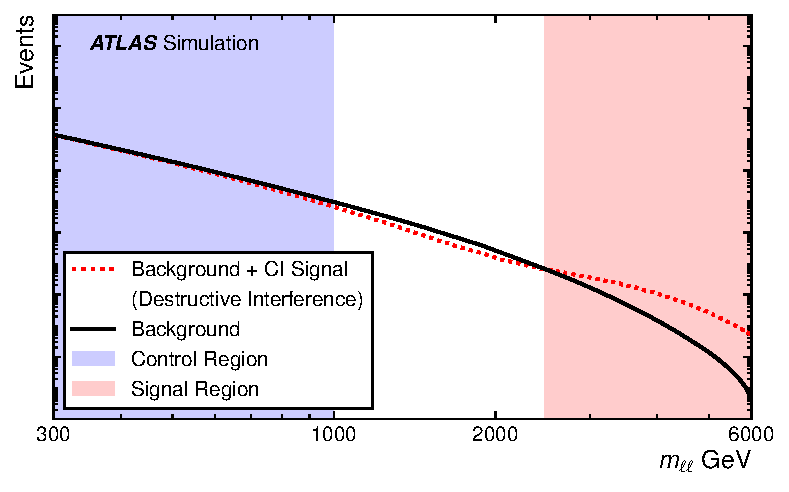
\includegraphics[width=0.8\textwidth]{/Users/Deshan/Documents/PhD/thesis/Thesis/figures/analysis/bkgmodel/fig_01a.pdf} 
    \caption[A schematic illustration of the possible mass ranges in this analysis.]{A schematic illustration of the possible mass ranges in this analysis.
    The monotonically falling total background shape is shown by the solid black line, while an example of a CI signal plus the total background shape is shown by the dotted red line. The CI signal is shown after the DY process has been subtracted to show only the interference and pure CI process.}
    \label{fig:bkgmodel:ranges}
\end{figure}

\section{Background fit function choice}\label{sec:modelchoice}
The background function is chosen from a variety of different candidates for its stability during the extrapolation procedure and the ability to accurately model the invariant mass distributions of the \ee and \mumu channels. Each function is fit to the background dilepton invariant mass template, produced by summing together the contributions from all the background processes, in a variety of different CRs and extrapolated to the corresponding SRs. The distribution of the pulls, defined as (fit-simulation)/fit, is obtained for each invariant mass bin for all initial CR and SR ranges considered. Functions which have pulls below 2 in the CR and SRs pass the initial selection. The functions are also required to have a flat distribution of pulls across the invariant-mass spectrum. These requirement ensures that functions which exhibit unphysical behaviour in the high-mass regions of the invariant mass spectrum are vetoed. Additionally, it ensures that good modelling of the simulated shape in the CR is maintained. There were a possible three functions which satisfied the above conditions. Regardless of the choice of final function, each function that satisfies the initial selection criteria will have inherent weaknesses in their bias and performance. These are then measured and taken into account as uncertainties, described in \cref{chap:uncertBkgmodel}. The final function was chosen out of the subset of functions to be consistent with the resonance analysis~\cite{Aad:2019fac}. The final fit function is given by
\begin{equation}
    \label{eq:fitfunc}
    \begin{aligned}
        & f_\textrm{b}(m_{\ell\ell}) = f_{\mathrm{BW},Z}(m_{\ell\ell}) \cdot \left(1 - x^{c}\right)^{b} \cdot x^{\sum_{i=0}^3 p_i\log(x)^i}, \\
        & f_{\mathrm{BW},Z}(\mathrm{m_{\ell\ell}}) = \frac{\Gamma_Z}{(m_Z - \mathrm{m_{\ell\ell}})^2 + \Gamma_Z^2},
    \end{aligned}
\end{equation}

where $x = m_{\ell\ell}/\sqrt{s}$, $f_{\mathrm{BW},Z}(m_{\ell\ell})$ is a non-relativistic Breit--Wigner function with $m_Z = \SI{91.1876}{\giga\electronvolt}$ and $\Gamma_Z = \SI{2.4952}{\giga\electronvolt}$~\cite{PhysRevD.98.030001}, $(1 - x^{c})^b$ ensures that the background fit evaluates to zero as $x \to 1$, to be consistent with the expectation from the collision energy of the LHC. Both b and c are constants that have been evaluated based on pre-fits performed on the full background template. The $p_i$ parameters, with $i = 0,1,2,3$, are left as free parameters to be informed by the fit. The term $x^{\sum_{i=0}^3 p_i\log(x)^i}$ has been studied in detail and accepted as a good approximation to model distributions with similar smoothly falling spectra~\cite{Aad:2019fac,Aaboud:2016tru,Aaboud:2017yyg}.

The fits to the data and simulation are both performed with a bin width of \SI{1}{\giga\electronvolt}. The function $f_b(m_{\ell\ell})$ is treated as a probability density in the fits performed to the CR. It is normalised in the CR to the number of events in the CR ($N_{CR}$) of the template being fit. \cref{fig:bkgmodel:fitstoMC} shows an example of background-only fits to the electron and muon channel in a CR and SR configuration. The plots are shown constant in $\log{(\text{m}_{\ell\ell})}$ binning for presentation purposes, as the linear binning used to perform the fits are difficult to interpret clearly. The figures show flat pulls below 1 for the electron and muon channels, indicating good modelling of the background distributions. 

\begin{figure}[h!]
    \centering
    \begin{subfigure}[b]{0.49\textwidth}
        \centering
        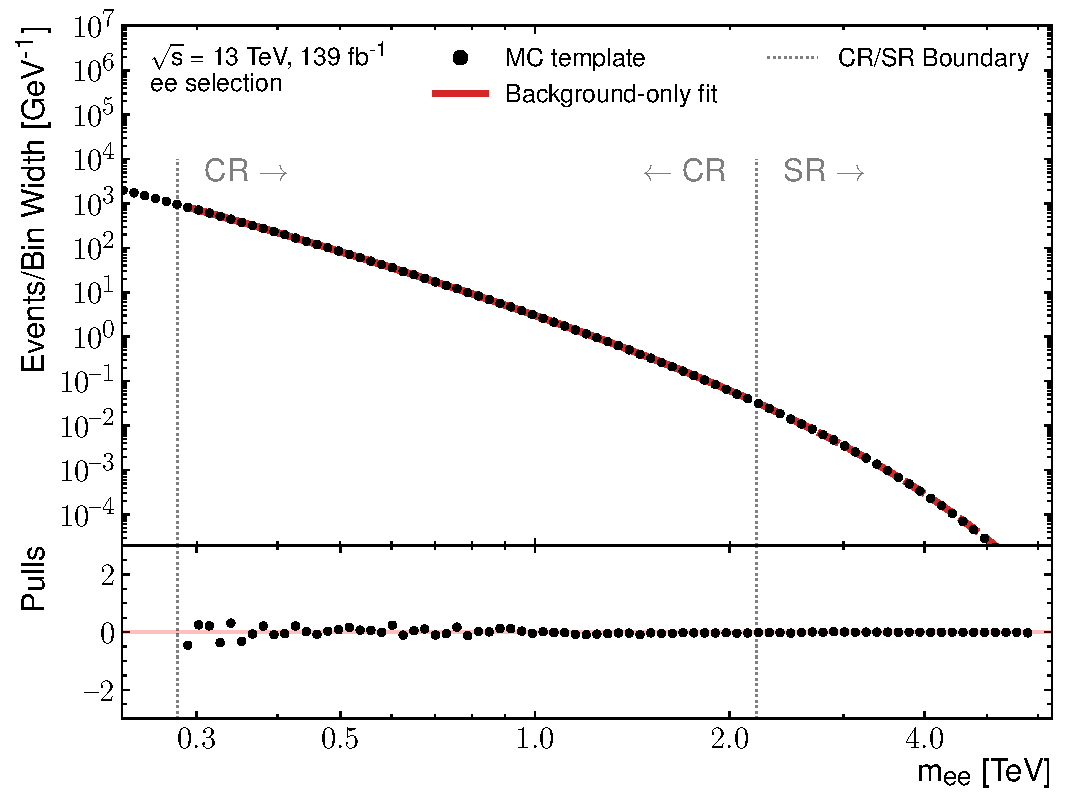
\includegraphics[width=\textwidth]{/Users/Deshan/Documents/PhD/thesis/Thesis/figures/analysis/bkgmodel/fit-const-ee-backgroundModel.pdf}
        \label{fig:fitstoMC1}
    \end{subfigure}
    \begin{subfigure}[b]{0.49\textwidth}
        \centering
        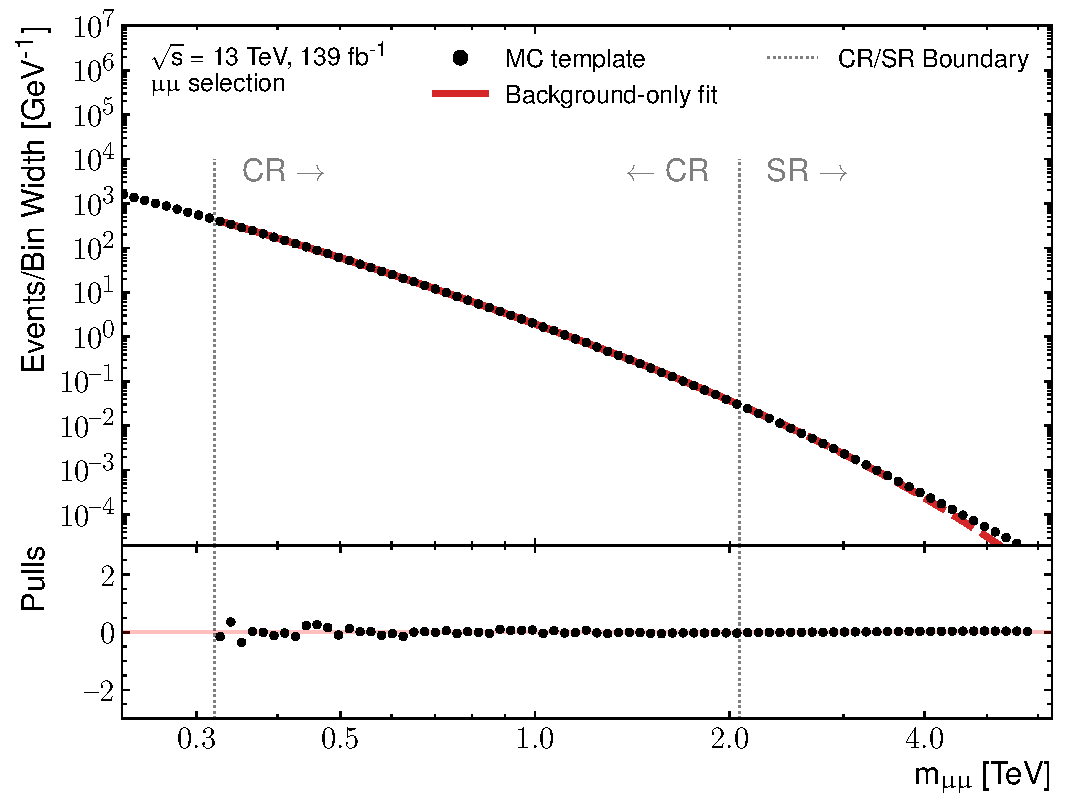
\includegraphics[width=\textwidth]{/Users/Deshan/Documents/PhD/thesis/Thesis/figures/analysis/bkgmodel/fit-const-mm-backgroundModel.pdf}
        \label{fig:fitstoMC2}
    \end{subfigure}
    \caption[Fits to the simulated background template in the electron and muon channels]{Fit to the simulated background template in the electron (left) and muon (right) channels shown in the top pad. The bottom pad shows the pulls of the fit. The CR and SR boundaries are also shown in the figure. The background template points are plotted at the centre of each bin as the number of events divided by the bin width, which is constant in $\log{(\text{m}_{\ell\ell})}$.}
    \label{fig:bkgmodel:fitstoMC}
\end{figure}

Examples of functions that were considered are given in \cref{tab:bkgmodel:functions}, with their corresponding fits to the data shown in \cref{fig:bkgmodel:badfitstomc}. \cref{fig:bkgmodel:fitstoMC3} depicts a function fit that is close to satisfying the function choice selection. However, it poorly models the extrapolated region compared to the function defined in \cref{eq:fitfunc}. \cref{fig:bkgmodel:fitstoMC4} shows a function that does not satisfy the the requirement that the pulls are below 1 and flat throughout the invariant mass distribution. Nonphysical behaviour in the fit and  extrapolation can be seen in \cref{fig:bkgmodel:fitstoMC5}. \cref{fig:bkgmodel:fitstoMC6} was not selected due to poor modelling of the CR. 

\begin{table}[h!]
    \centering
    \begin{tabular}{c|l}
         & Function definition \\
        \hline\hline 
        1 & $(1 - x^{5})^{\text{p0}}*(x^{(\text{p1} + \text{p2}*\log(x)})$ \\
        2 & $(1-\log(e*x^{\text{p1}})+c1*x*e^{\text{p2}/(1+x^{\text{p3}})}$ \\
        3 & $(x)^{\text{p1}}*e^{\text{p2}*x}$\\
        4 & $(1-x)^{\text{p1}}*e^{\text{p2}*x^2}$ \\
    \end{tabular}
    \caption[List of functions considered for the background fit]{List of functions considered for fit to dilepton spectrum that did not pass the criteria required. $x$ is defined to be $= m_{\ell\ell}/\sqrt{s}$. }
    \label{tab:bkgmodel:functions}
\end{table}

\begin{figure}[h!]
    \centering
    \begin{subfigure}[b]{0.49\textwidth}
        \centering
        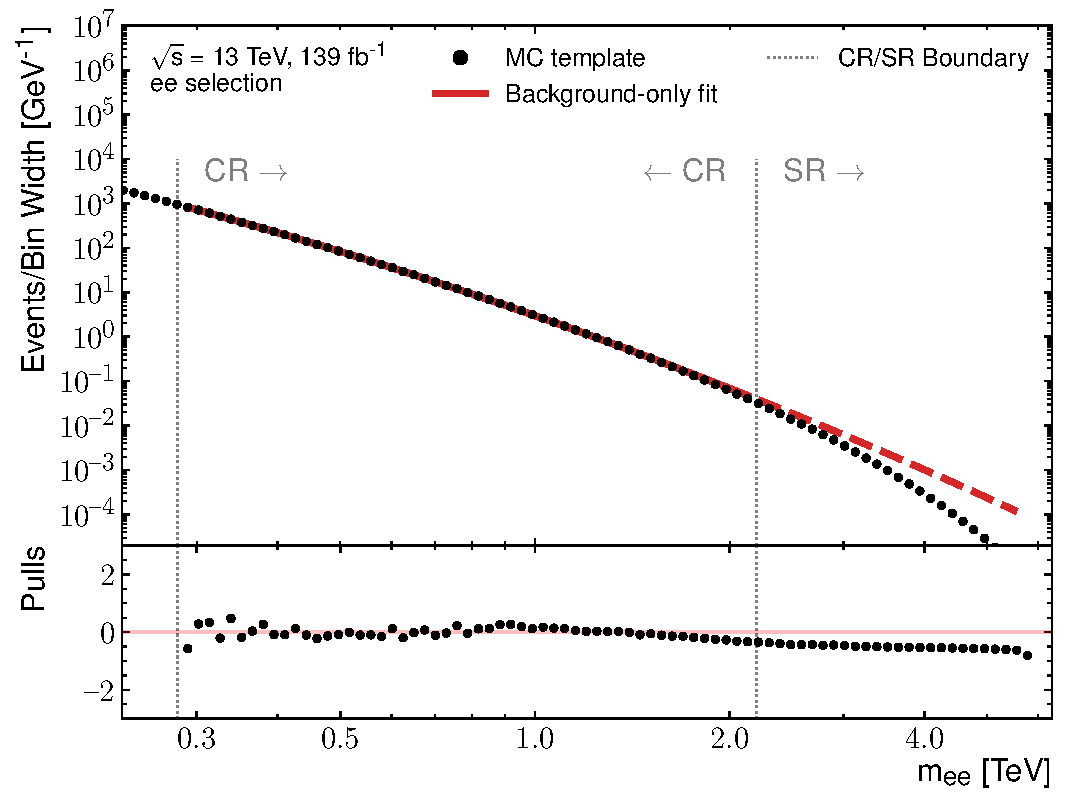
\includegraphics[width=\textwidth]{/Users/Deshan/Documents/PhD/thesis/Thesis/figures/analysis/bkgmodel/fit-const-ee-diphoton3.pdf}
        \caption{}
        \label{fig:bkgmodel:fitstoMC3}
    \end{subfigure}
    \begin{subfigure}[b]{0.49\textwidth}
        \centering
        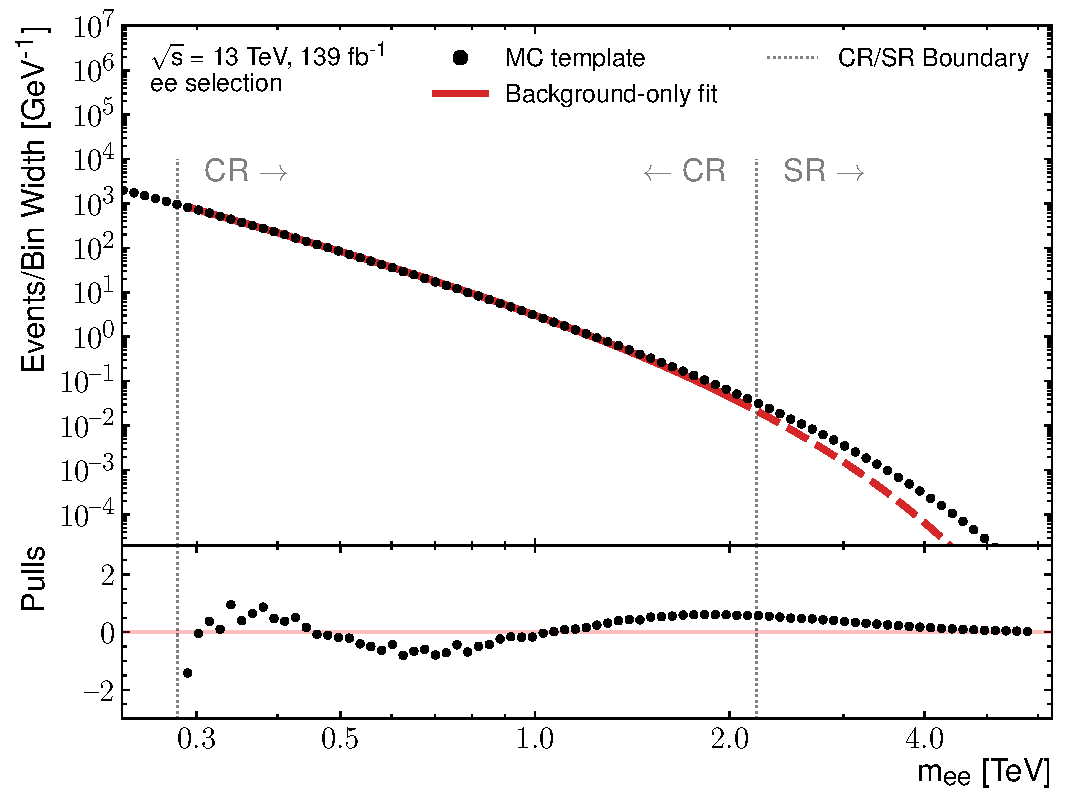
\includegraphics[width=\textwidth]{/Users/Deshan/Documents/PhD/thesis/Thesis/figures/analysis/bkgmodel/fit-const-ee-dext1.pdf}
        \caption{}
        \label{fig:bkgmodel:fitstoMC4}
    \end{subfigure}
    \begin{subfigure}[b]{0.49\textwidth}
        \centering
        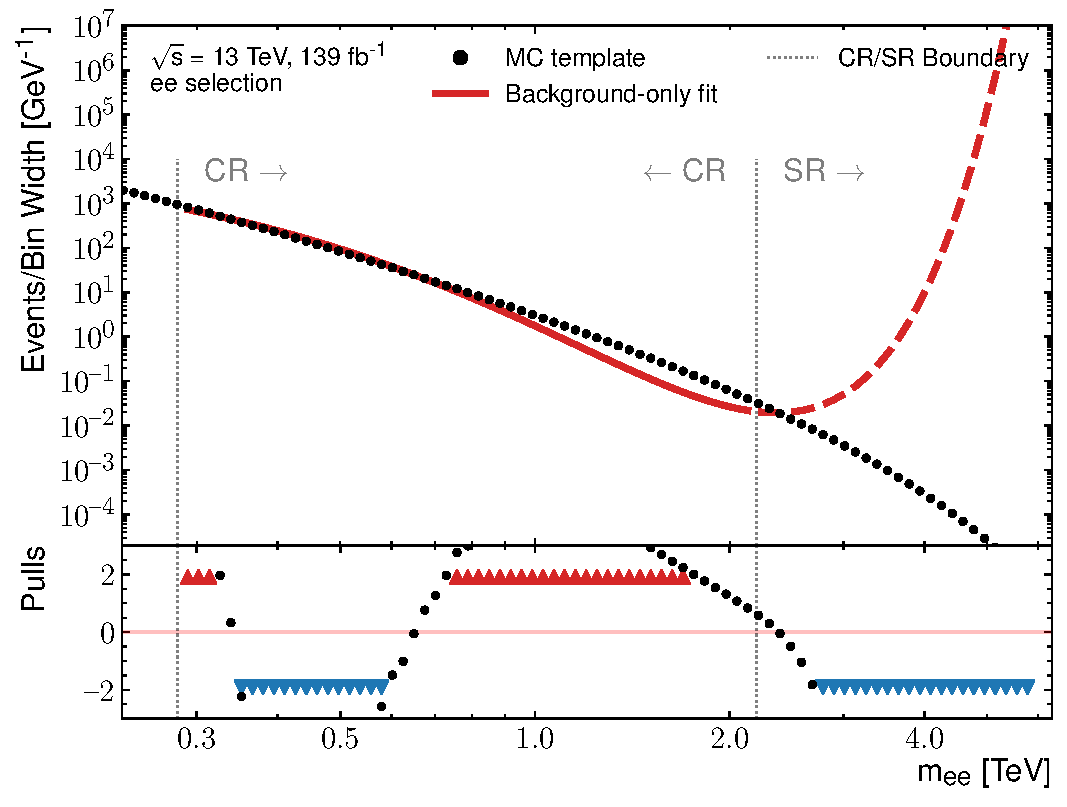
\includegraphics[width=\textwidth]{/Users/Deshan/Documents/PhD/thesis/Thesis/figures/analysis/bkgmodel/fit-const-ee-multijetf2.pdf}
        \caption{}
        \label{fig:bkgmodel:fitstoMC5}
    \end{subfigure}
    \begin{subfigure}[b]{0.49\textwidth}
        \centering
        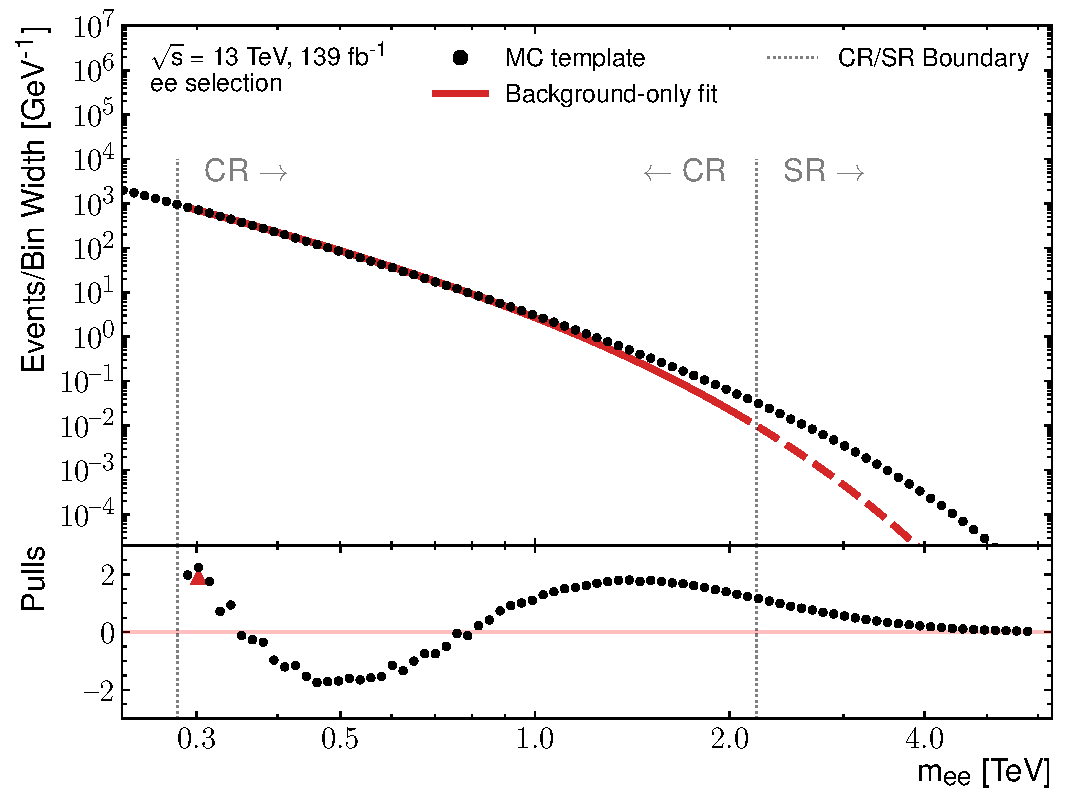
\includegraphics[width=\textwidth]{/Users/Deshan/Documents/PhD/thesis/Thesis/figures/analysis/bkgmodel/fit-const-ee-UA2_1.pdf}
        \caption{}
        \label{fig:bkgmodel:fitstoMC6}
    \end{subfigure}
    \caption[Fits to the simulated background template in the electron and muon channels using functions that did not pass the selection criteria]{Fits using functions that failed the function choice criteria, to the simulated background template in the electron channel shown in the top pad. Figures (a), (b), (c) and (d) correspond to functions 1, 2, 3, and 4 in \cref{tab:bkgmodel:functions}, respectively. The bottom pad shows the pulls of the fit. The CR and SR boundaries are also shown in the figure. The background template points are plotted at the centre of each bin as the number of events divided by the bin width, which is constant in $\log{(\text{m}_{\ell\ell})}$.}
    \label{fig:bkgmodel:badfitstomc}
\end{figure}
\clearpage

\section{Signal+background function}\label{sec:sigmodel}
The CR choice is validated using a signal+background function in order to avoid bias from possible signal contamination in the CR. The signal+background function is used in \emph{signal injection} tests and to validate the background-only function once the CR and SR choice has been finalised. The signal injection tests are used in the optimisation process, described in \cref{sec:extrap:optimisation}, in order to choose a CR and SR configuration that will not be biased by the presence of signals. A collection of signal samples at various $\Lambda$ values are injected into the background template, and the effect on the background estimation from the fit and extrapolation is checked. The signal+background function is formed by adding a signal component is added to \cref{eq:fitfunc} to give
\begin{equation}
    \label{eq:sbfunction}
    \begin{aligned}
    f_\textrm{b+s}(m_{\ell\ell},\Lambda) = N_\textrm{b}\cdot f_\textrm{b}(m_{\ell\ell}) + N_\textrm{s}(\Lambda)\cdot f_\textrm{s}(m_{\ell\ell},\Lambda),
    \end{aligned} 
\end{equation}
where $f_\textrm{s}(m_{\ell\ell},\Lambda)$ is the signal probability density function and $N_\textrm{s}(\Lambda)$ is the number of signal events in the CR. Both $f_\textrm{s}(m_{\ell\ell},\Lambda)$ and $N_\textrm{s}(\Lambda)$ are determined from simulation. The morphing procedure, described in \cref{sec:datamc:mc:sig:morphing}, is used to obtain a smooth description of a given CI model as function of $\Lambda$, allowing to determine the signal contribution that fall between the fixed signal shapes from simulation. The parameter $N_\textrm{b}$ is the number of background events in the CR, where the total number of events in the CR is given by $N_\textrm{b}+N_\textrm{s}(\Lambda)=N_\textrm{CR}$. 

\cref{fig:bkgmodel:sbfits} depicts signal+background fits to a background template injected with a CI interaction signal at $\Lambda = \SI{26}{\tera\electronvolt}$ in the electron and muon channels. The background component of the signal+background fit is separated and compared with the background template, and the pulls are calculated. The figure shows that the background component of the signal+background fit is not biased by the presence of a signal in the CR. 
\begin{figure}[h!]
    \centering
    \begin{subfigure}[b]{0.49\textwidth}
        \centering
        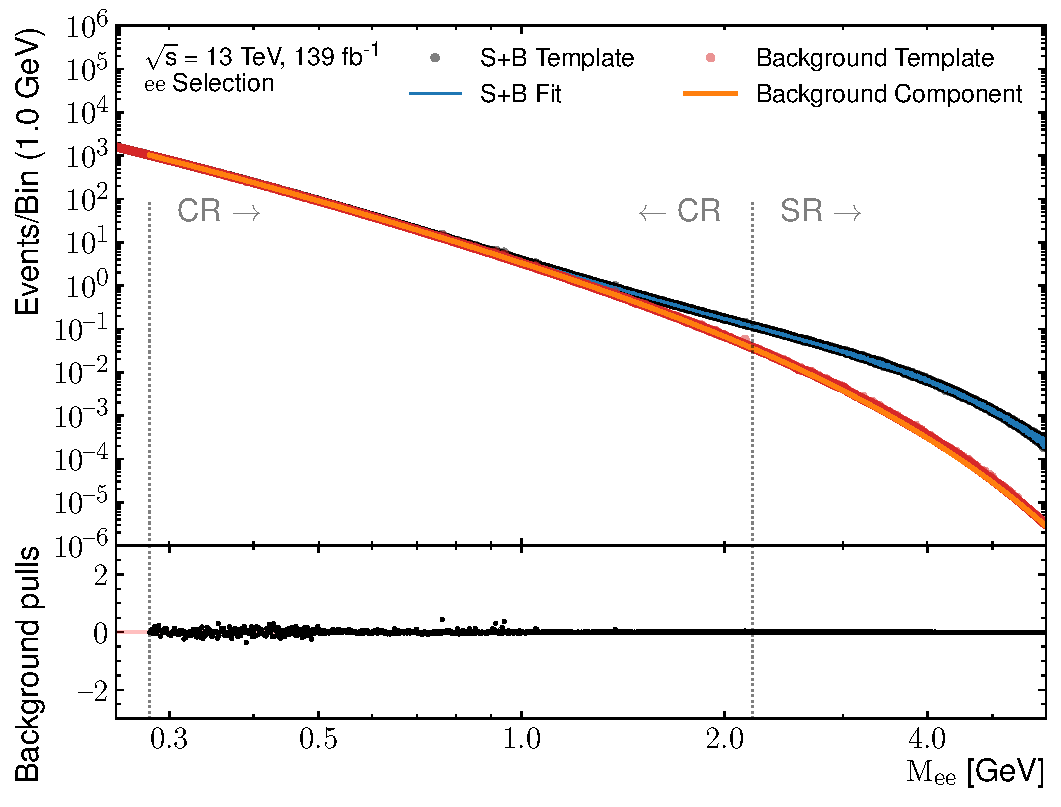
\includegraphics[width=\textwidth]{/Users/Deshan/Documents/PhD/thesis/Thesis/figures/analysis/bkgmodel/nominalFit-sb-const-LL-18-sbTrue-ee-.pdf}
        \label{fig:bkgmodel:sbfits1}
    \end{subfigure}
    \begin{subfigure}[b]{0.49\textwidth}
        \centering
        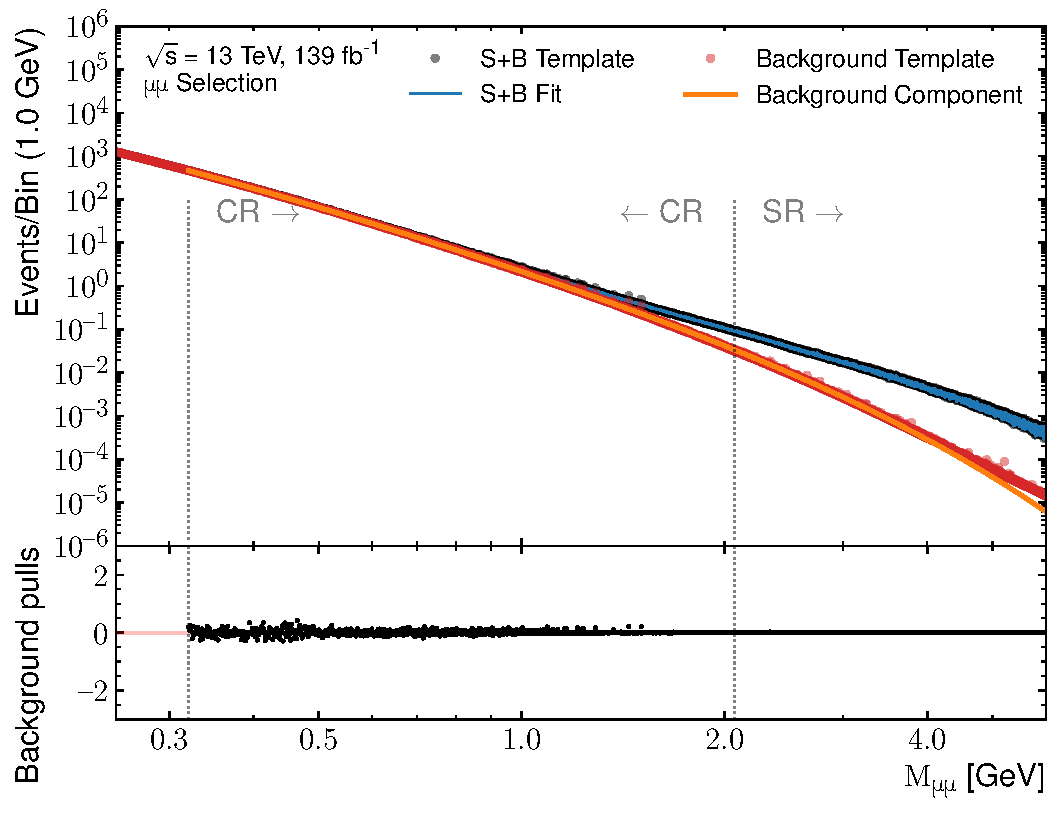
\includegraphics[width=\textwidth]{/Users/Deshan/Documents/PhD/thesis/Thesis/figures/analysis/bkgmodel/nominalFit-sb-const-LL-18-sbTrue-mm-.pdf}
        \label{fig:bkgmodel:sbfits2}
    \end{subfigure}
    \caption[Signal+Background fits to the signal+background template in the electron and muon channels]{Signal+background (S+B) fit to the simulated template injected with a CI signal at $\Lambda = \SI{26}{\tera\electronvolt}$ in the electron (left) and muon (right) channels shown in the top pad. The background template and the background component of the S+B fit corresponds to the blue and red lines, respectively. The background template (red data-points) is injected with a CI signal to form the signal+background template (blue data-points). The bottom pad shows the pulls of the background component of the fit compared to the background template. The CR and SR boundaries are shown in the figure.}
    \label{fig:bkgmodel:sbfits}
\end{figure}

\subsection{Signal injection tests}\label{sec:extrap:recovery}
Signal injection tests are used to validate the requirement that the signal+background function can provide an accurate background estimate, regardless of the presence of a signal in the CR. The robustness of the signal+background function is validated by quantifying the deflection of the function in the presence of an injected signal in the template. The signal+background function is fit to signal+background MC templates, consisting of the MC background-only template injected with CI models in a range of $\Lambda$ values. The background expectation from the signal+background function is compared to the background-only MC template in these tests. 

\cref{fig:bkgmodel:injeeconst,fig:bkgmodel:injmmconst,fig:bkgmodel:injeedest,fig:bkgmodel:injmmdest} depict the injection tests in the electron and muon channel for the different chiral and interference models considered. The final CR and SR choices are used to depict the performance of the signal+background function. The figures show that the background estimate from the signal+background function fit does not change significantly in the presence of injected CI signals, and is consistent with the background estimate from fitting the background-only MC template. Statistical fluctuations in the injected signals cause small discrepancies between background estimates, for e.g. \cref{fig:bkgmodel:injeeconst}. Additionally, the presence of a destructive interference CI signal can result in the function under-fitting the background distribution, resulting in a lower estimated background compared the fit without an injected signal. This is due to the destructive component of the interference model. However, the effect is small and well within the uncertainties of the estimated background. The signals are injected from $\Lambda = \SI{18}{\tera\electronvolt}$ to \SI{40}{\tera\electronvolt}. 

\begin{figure}[h!]
    \centering
    \begin{subfigure}[b]{0.49\textwidth}
        \centering
        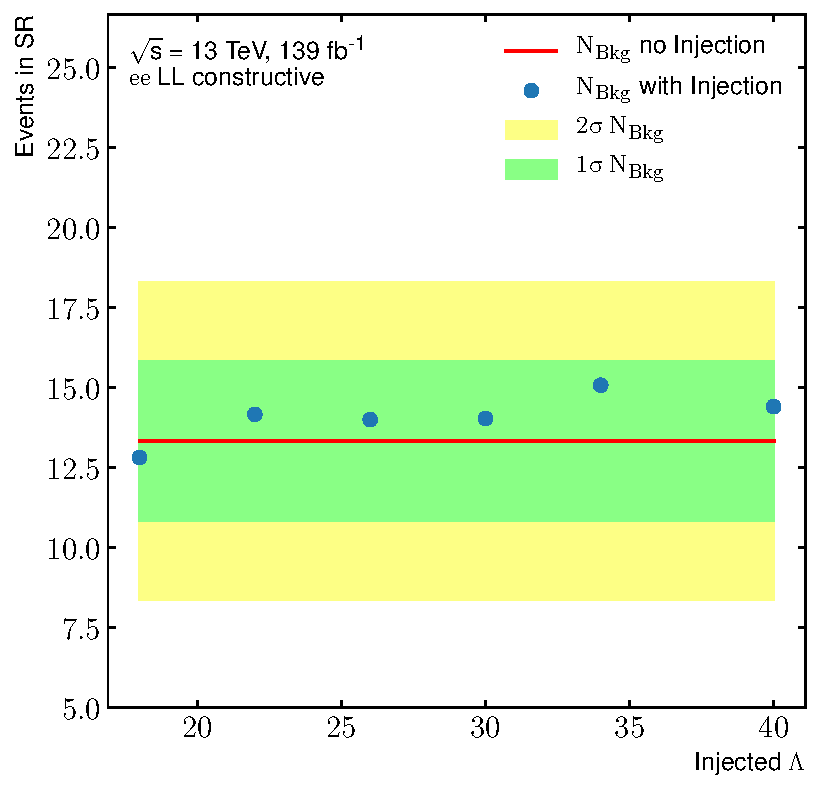
\includegraphics[width=\textwidth]{/Users/Deshan/Documents/PhD/thesis/Thesis/figures/analysis/bkgmodel/injections/injFlat-const-LL-ee.pdf}
        \label{fig:bkgmodel:injee1}
    \end{subfigure}
    \begin{subfigure}[b]{0.49\textwidth}
        \centering
        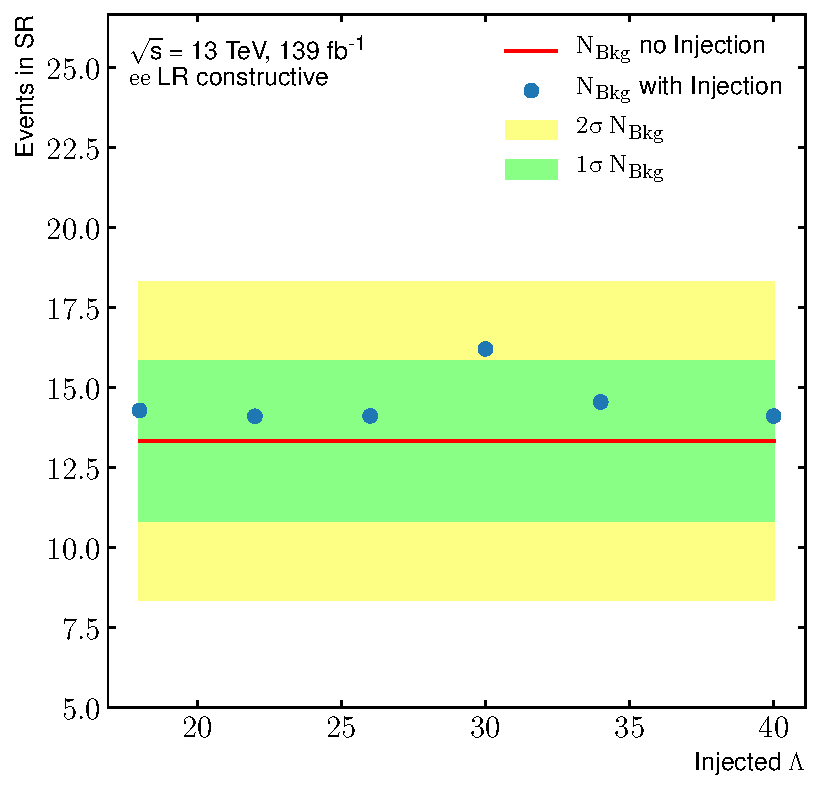
\includegraphics[width=\textwidth]{/Users/Deshan/Documents/PhD/thesis/Thesis/figures/analysis/bkgmodel/injections/injFlat-const-LR-ee.pdf}
        \label{fig:bkgmodel:injee3}
    \end{subfigure}
    \begin{subfigure}[b]{0.49\textwidth}
        \centering
        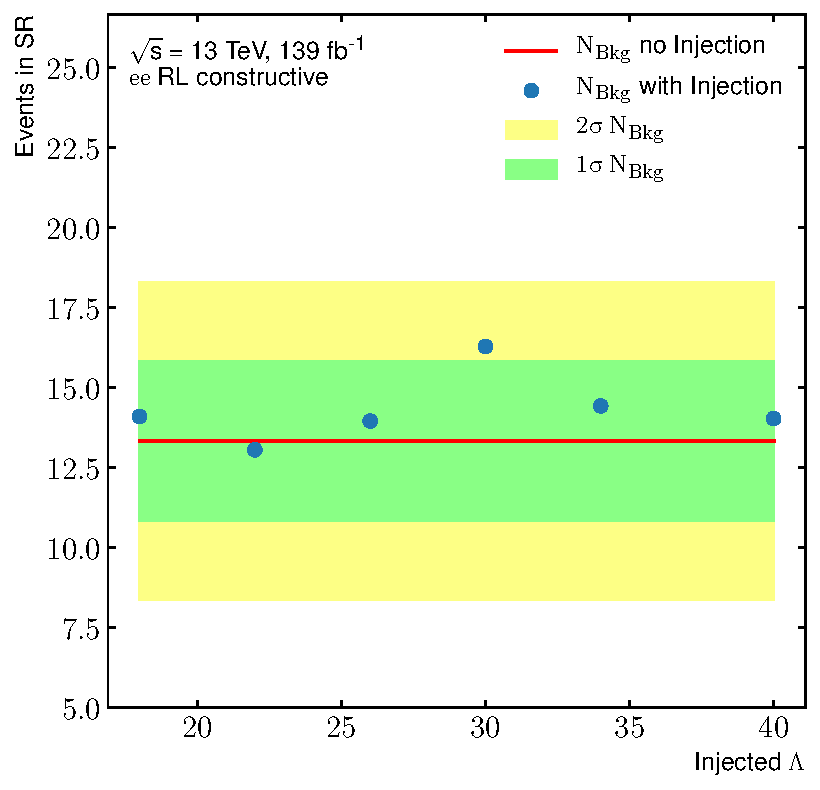
\includegraphics[width=\textwidth]{/Users/Deshan/Documents/PhD/thesis/Thesis/figures/analysis/bkgmodel/injections/injFlat-const-RL-ee.pdf}
        \label{fig:bkgmodel:injee5}
    \end{subfigure}
    \begin{subfigure}[b]{0.49\textwidth}
        \centering
        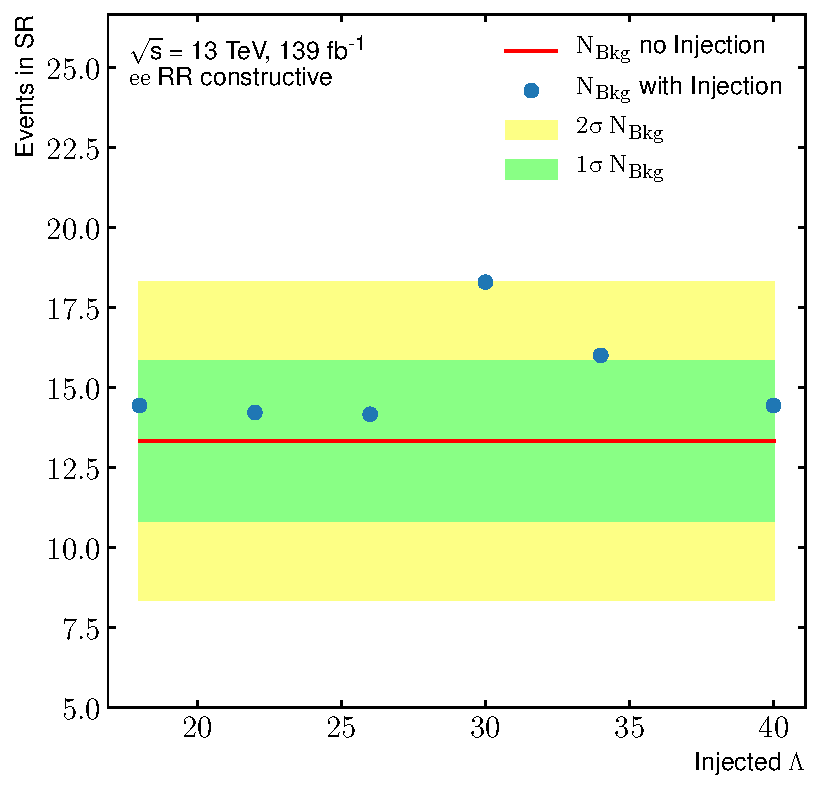
\includegraphics[width=\textwidth]{/Users/Deshan/Documents/PhD/thesis/Thesis/figures/analysis/bkgmodel/injections/injFlat-const-RR-ee.pdf}
        \label{fig:bkgmodel:injee7}
    \end{subfigure}
    \caption[Signal injection tests in the electron channel for constructive interference models]{Signal injection tests in the electron channel. The background expectation in the SR for the signal+background function is compared for fits to the background template with injections of various chiral CI signals from $\Lambda = \SI{18}{\tera\electronvolt}$ to \SI{40}{\tera\electronvolt}. The LL, LR, RL, and RR chiral constructive interference models are injected. The background estimation from the fit to the background MC template with its associated uncertainty is also shown.}
    \label{fig:bkgmodel:injeeconst}
\end{figure}

\begin{figure}[h!]
    \centering
    \begin{subfigure}[b]{0.49\textwidth}
        \centering
        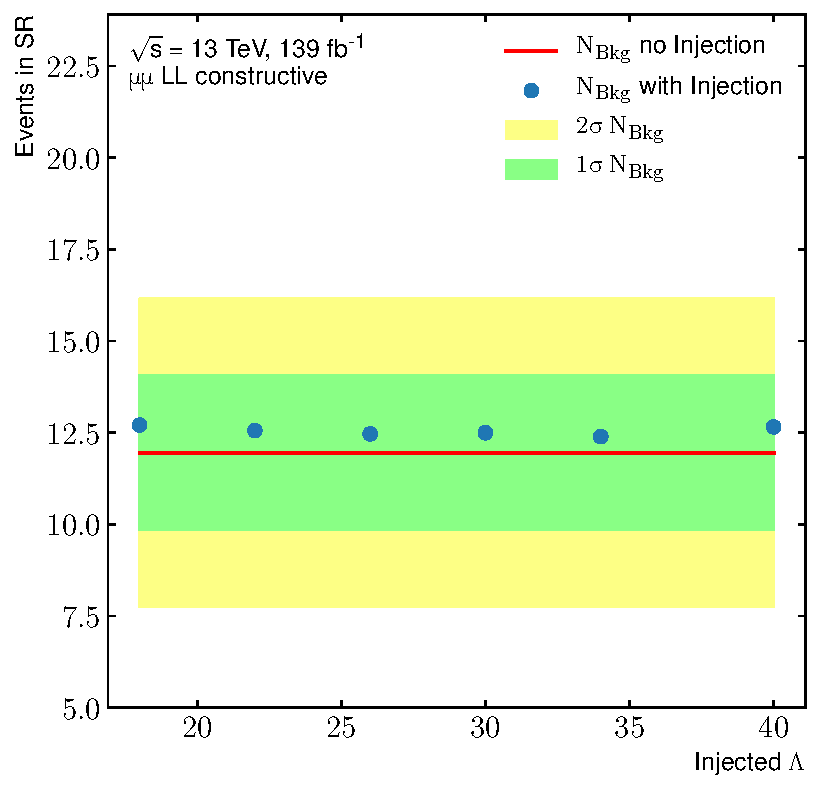
\includegraphics[width=\textwidth]{/Users/Deshan/Documents/PhD/thesis/Thesis/figures/analysis/bkgmodel/injections/injFlat-const-LL-mm.pdf}
        \label{fig:bkgmodel:injmm1}
    \end{subfigure}
    \begin{subfigure}[b]{0.49\textwidth}
        \centering
        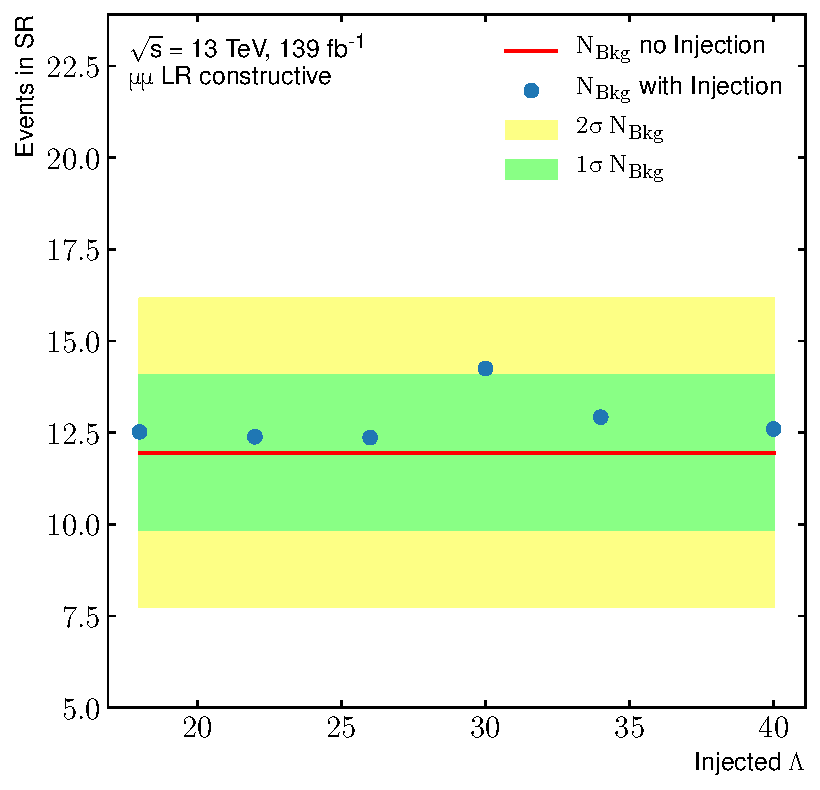
\includegraphics[width=\textwidth]{/Users/Deshan/Documents/PhD/thesis/Thesis/figures/analysis/bkgmodel/injections/injFlat-const-LR-mm.pdf}
        \label{fig:bkgmodel:injmm3}
    \end{subfigure}
    \begin{subfigure}[b]{0.49\textwidth}
        \centering
        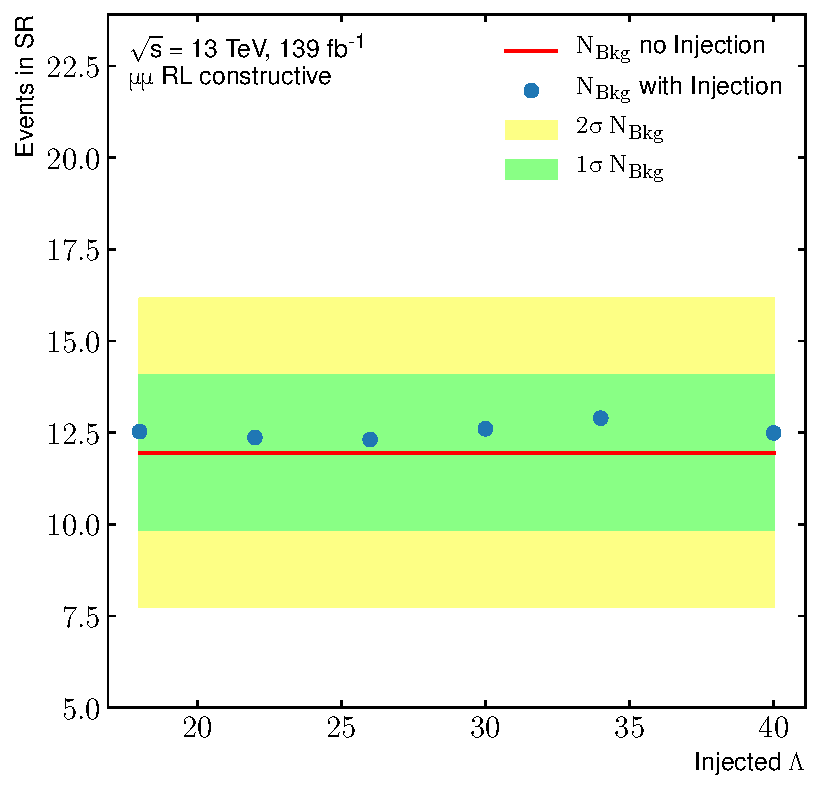
\includegraphics[width=\textwidth]{/Users/Deshan/Documents/PhD/thesis/Thesis/figures/analysis/bkgmodel/injections/injFlat-const-RL-mm.pdf}
        \label{fig:bkgmodel:injmm5}
    \end{subfigure}
    \begin{subfigure}[b]{0.49\textwidth}
        \centering
        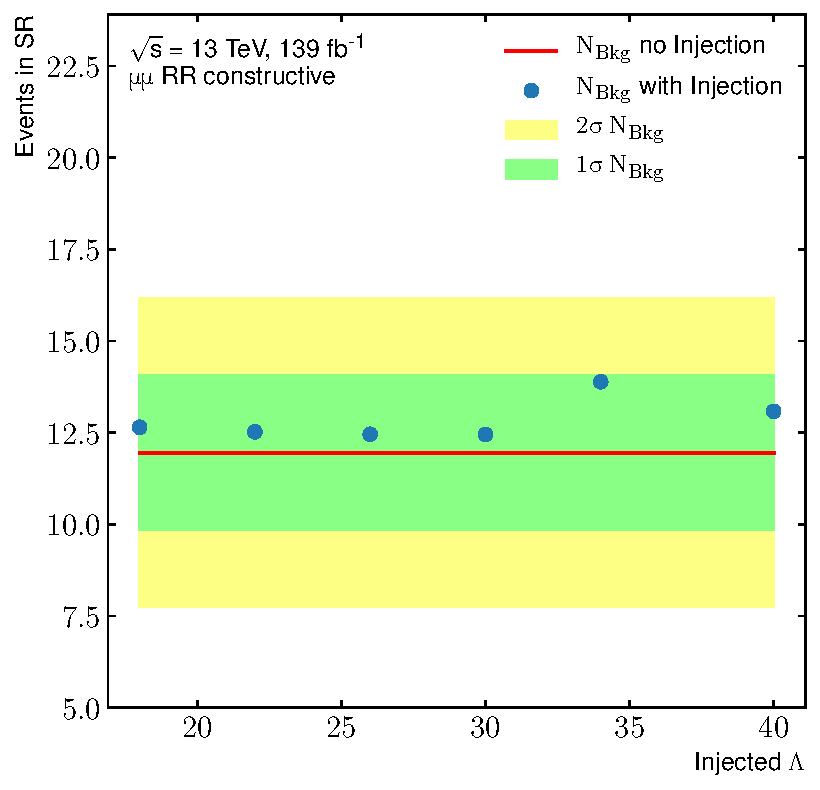
\includegraphics[width=\textwidth]{/Users/Deshan/Documents/PhD/thesis/Thesis/figures/analysis/bkgmodel/injections/injFlat-const-RR-mm.pdf}
        \label{fig:bkgmodel:injmm7}
    \end{subfigure}
    \caption[Signal injection tests in the muon channel for destructive interference models]{Signal injection tests in the muon channel. The background expectation in the SR for the signal+background function is compared for fits to the background template with injections of various chiral CI signals from $\Lambda = \SI{18}{\tera\electronvolt}$ to \SI{40}{\tera\electronvolt}. The LL, LR, RL, and RR chiral destructive interference models are injected. The background estimation from the fit to the background MC template with its associated uncertainty is also shown.}
    \label{fig:bkgmodel:injmmconst}
\end{figure}

\begin{figure}[h!]
    \centering
    \begin{subfigure}[b]{0.49\textwidth}
        \centering
        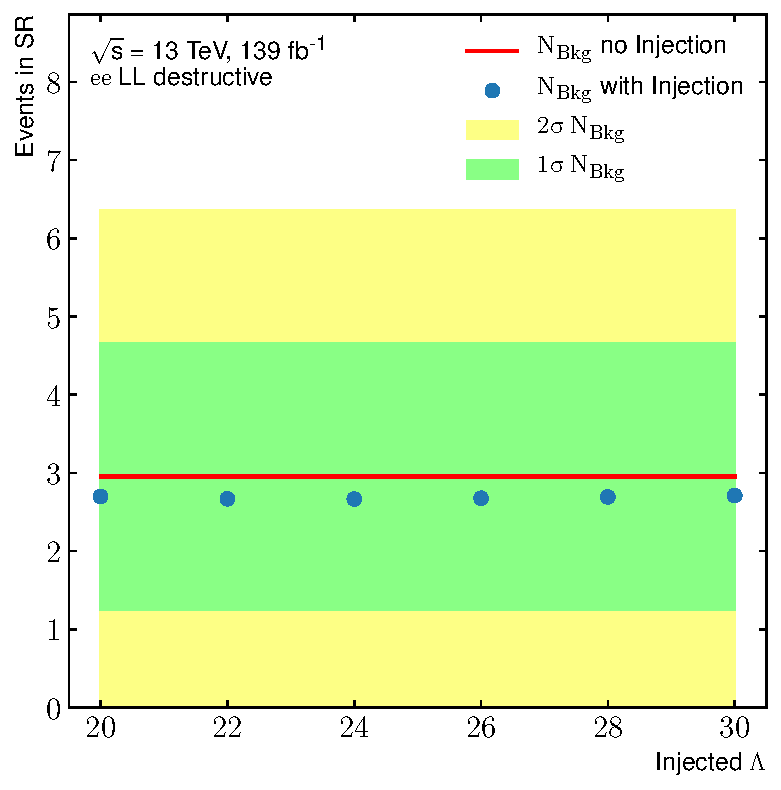
\includegraphics[width=\textwidth]{/Users/Deshan/Documents/PhD/thesis/Thesis/figures/analysis/bkgmodel/injections/injFlat-dest-LL-ee.pdf}
        \label{fig:bkgmodel:injee2}
    \end{subfigure}
    \begin{subfigure}[b]{0.49\textwidth}
        \centering
        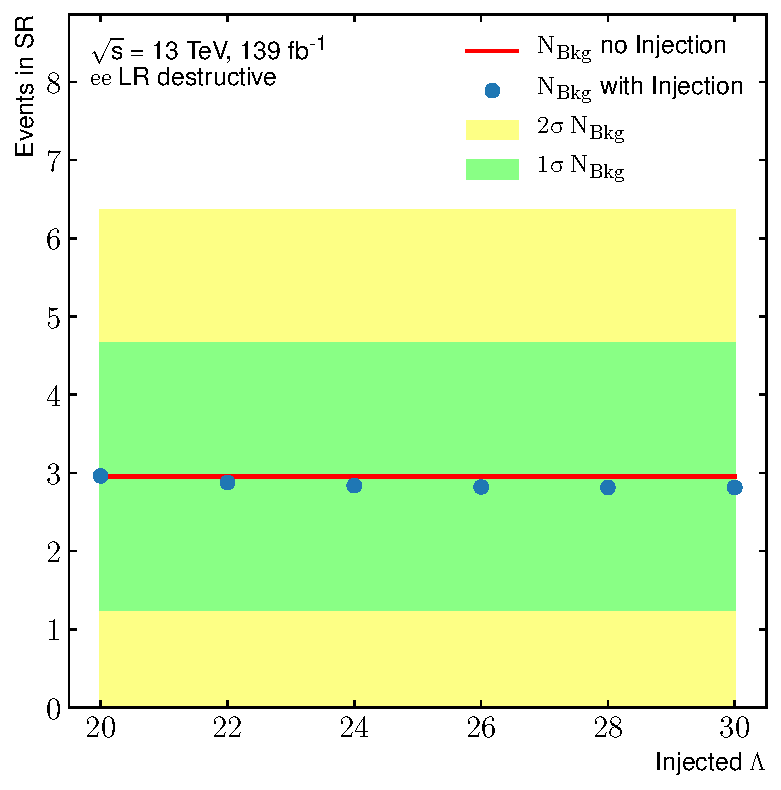
\includegraphics[width=\textwidth]{/Users/Deshan/Documents/PhD/thesis/Thesis/figures/analysis/bkgmodel/injections/injFlat-dest-LR-ee.pdf}
        \label{fig:bkgmodel:injee4}
    \end{subfigure}
    \begin{subfigure}[b]{0.49\textwidth}
        \centering
        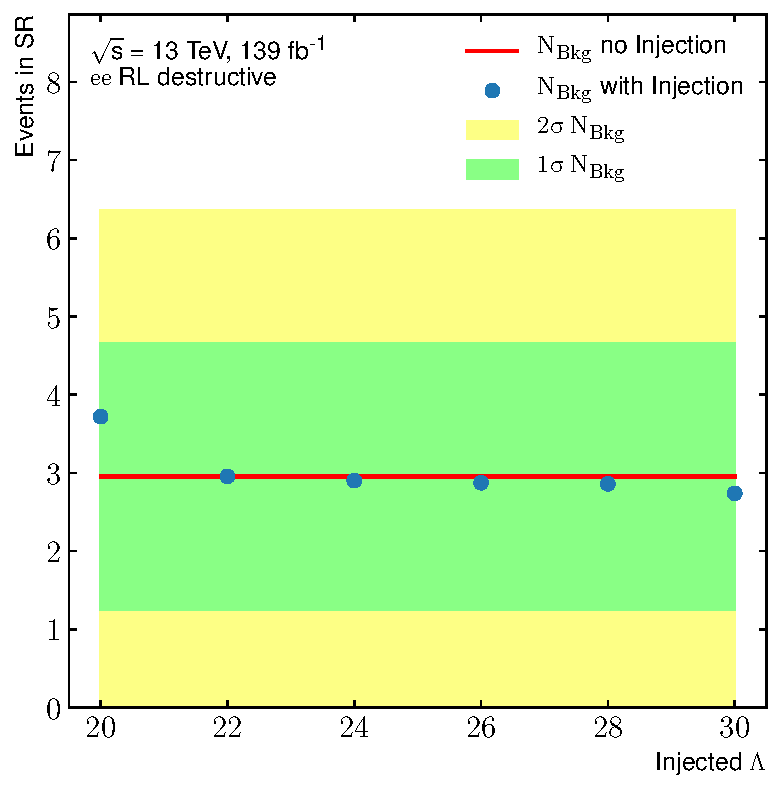
\includegraphics[width=\textwidth]{/Users/Deshan/Documents/PhD/thesis/Thesis/figures/analysis/bkgmodel/injections/injFlat-dest-RL-ee.pdf}
        \label{fig:bkgmodel:injee6}
    \end{subfigure}
    \begin{subfigure}[b]{0.49\textwidth}
        \centering
        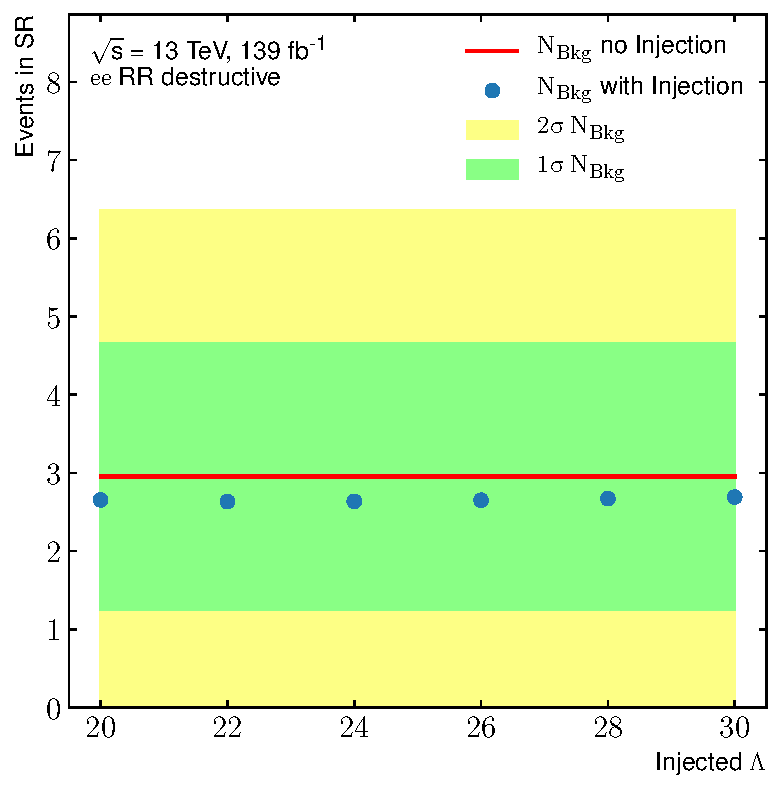
\includegraphics[width=\textwidth]{/Users/Deshan/Documents/PhD/thesis/Thesis/figures/analysis/bkgmodel/injections/injFlat-dest-RR-ee.pdf}
        \label{fig:bkgmodel:injee8}
    \end{subfigure}
    \caption[Signal injection tests in the electron channel for destructive interference models]{Signal injection tests in the electron channel. The background expectation in the SR for the signal+background function is compared for fits to the background template with injections of various chiral CI signals from $\Lambda = \SI{18}{\tera\electronvolt}$ to \SI{40}{\tera\electronvolt}. The LL, LR, RL, and RR chiral constructive interference models are injected. The background estimation from the fit to the background MC template with its associated uncertainty is also shown.}
    \label{fig:bkgmodel:injeedest}
\end{figure}

\begin{figure}[h!]
    \centering
    \begin{subfigure}[b]{0.49\textwidth}
        \centering
        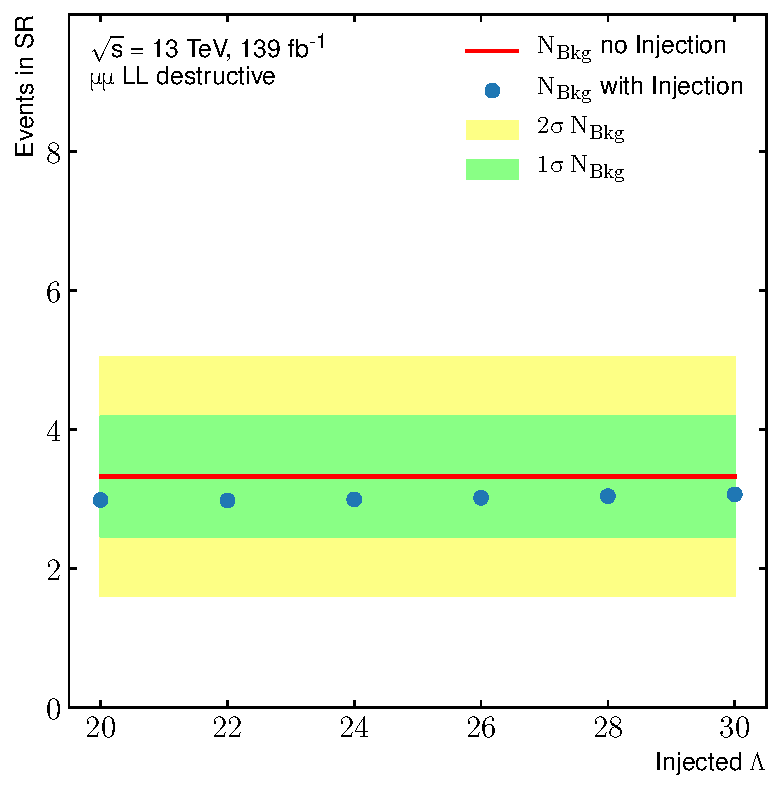
\includegraphics[width=\textwidth]{/Users/Deshan/Documents/PhD/thesis/Thesis/figures/analysis/bkgmodel/injections/injFlat-dest-LL-mm.pdf}
        \label{fig:bkgmodel:injmm2}
    \end{subfigure}
    \begin{subfigure}[b]{0.49\textwidth}
        \centering
        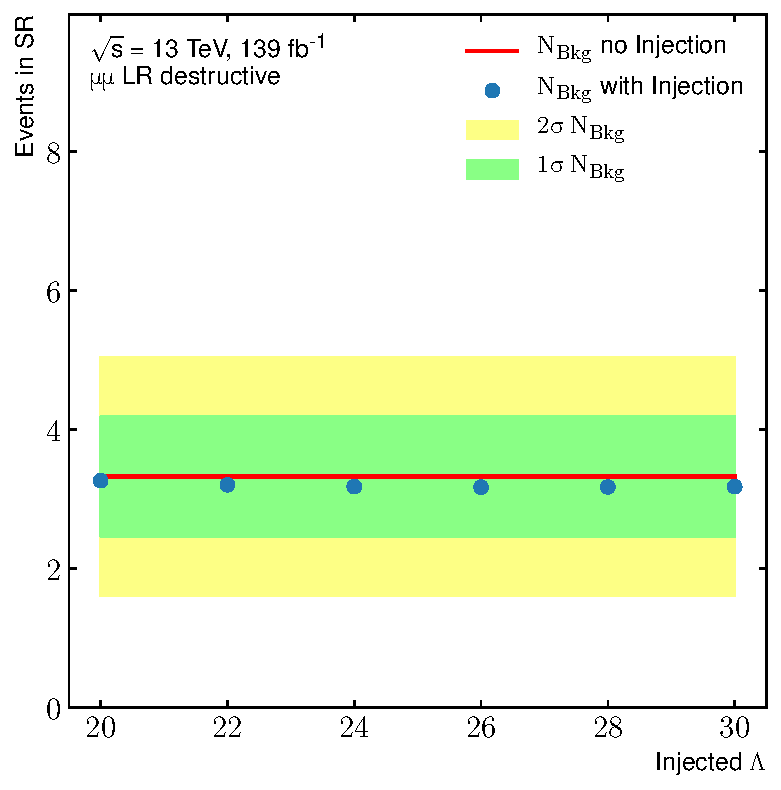
\includegraphics[width=\textwidth]{/Users/Deshan/Documents/PhD/thesis/Thesis/figures/analysis/bkgmodel/injections/injFlat-dest-LR-mm.pdf}
        \label{fig:bkgmodel:injmm4}
    \end{subfigure}
    \begin{subfigure}[b]{0.49\textwidth}
        \centering
        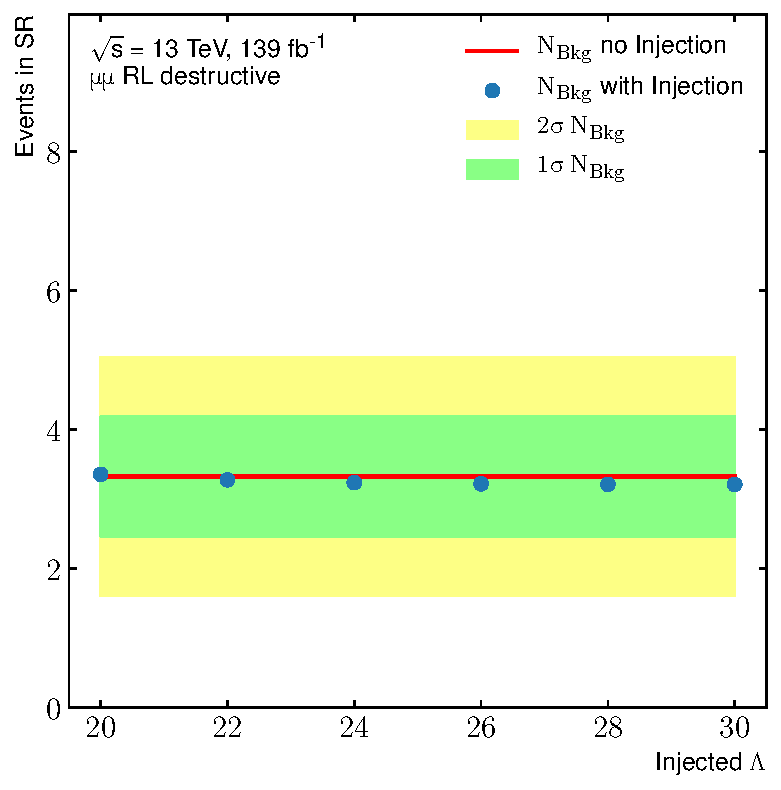
\includegraphics[width=\textwidth]{/Users/Deshan/Documents/PhD/thesis/Thesis/figures/analysis/bkgmodel/injections/injFlat-dest-RL-mm.pdf}
        \label{fig:bkgmodel:injmm6}
    \end{subfigure}
    \begin{subfigure}[b]{0.49\textwidth}
        \centering
        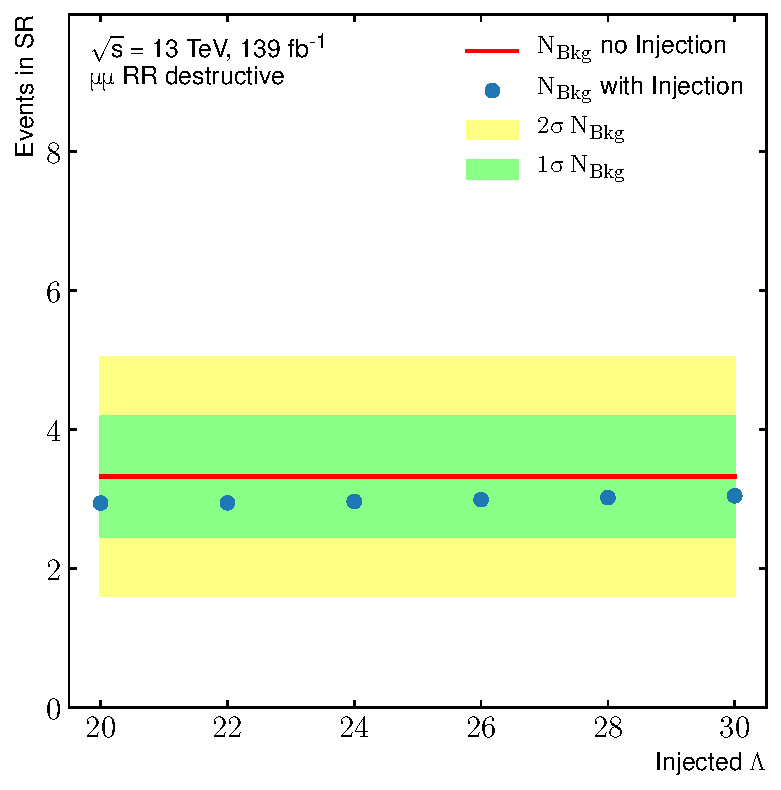
\includegraphics[width=\textwidth]{/Users/Deshan/Documents/PhD/thesis/Thesis/figures/analysis/bkgmodel/injections/injFlat-dest-RR-mm.pdf}
        \label{fig:bkgmodel:injmm8}
    \end{subfigure}
    \caption[Signal injection tests in the muon channel for destructive interference models]{Signal injection tests in the muon channel. The background expectation in the SR for the signal+background function is compared for fits to the background template with injections of various chiral CI signals from $\Lambda = \SI{18}{\tera\electronvolt}$ to \SI{40}{\tera\electronvolt}. The LL, LR, RL, and RR chiral constructive interference models are injected. The background estimation from the fit to the background MC template with its associated uncertainty is also shown.}
    \label{fig:bkgmodel:injmmdest}
\end{figure}

\clearpage
\section{Optimisation of control and signal regions}\label{sec:extrap:optimisation}
The optimisation procedure attempts to maximise the expected sensitivity to CI signals by varying the CR and SR boundaries. For each CI signal model and channel in consideration the lower and upper boundary of the CR ($\mathrm{CR}_{\mathrm{min}}$ and $\mathrm{CR}_{\mathrm{max}}$), and the lower boundary of the SR ($\mathrm{SR}_{\mathrm{min}}$) are varied to maximise sensitivity to CI signals. 

The expected limit is used to test the sensitivity to the CI models. The expected limit includes the background uncertainties, described in \cref{chap:uncertBkgmodel}, and is included in the statistical model following the procedure described in \cref{chap:stats}. An optimisation based solely on the expected limit would prefer CRs that extend to higher masses, as shown in \cref{chap:uncertBkgmodel}. However, extending the CR to high invariant-mass may result in a possible bias to the background expectation from signals present in data. This is addressed by introducing a second criteria based on minimising the linearity of the signal injection tests. The linearity criteria considers the performance of the recovery of signal events across a range of plausible CI signals injected to the MC background template, and is defined as
\begin{equation}
    \label{eq:linearity}
    \begin{aligned}
        \mathrm{Linearity} = \sum^{\Lambda = 18}_{\Lambda = \infty} \frac{N_{S,\mathrm{rec},\Lambda}}{N_{S,\mathrm{inj},\Lambda}}  \frac{1}{\mathrm{N}_\mathrm{tot}},
    \end{aligned}
\end{equation}

where $\Lambda$ is the CI energy scale in the injected MC template that is fit, $\Lambda = \infty$ corresponds to the background-only MC template, while $\Lambda = 18$ corresponds to a \SI{18}{\tera\electronvolt} CI signal injected. $N_{S,\mathrm{inj},\Lambda}$ is the number of injected signal events in the SR, $N_{S,\mathrm{rec},\Lambda}$ corresponds to the recovered number of signals events, defined as the difference between integrals of the signal+background template that is fit and the background expectation of the fit and extrapolation in the SR, $\mathrm{N}_\mathrm{tot}$ is the number of different signals that are injected, used to normalise the linearity to unity. The signal+background function is used for the linearity tests. 

A combination of both the expected limit and the linearity is used to pick a final CR and SR configuration. A balance between the expected limit and linearity is required for an optimal CR and SR configuration. The different chiral and interference CI signal models are considered in the optimisation. The chiral models correspond to LL, LR, RL, and RR, and the interference models considered are either constructive or destructive. In the destructive interference cases, if the SR includes a significant contribution from the destructive interference component of the CI signal shape, the integral number of expected events in the SR is reduced. Therefore, the optimisation procedure allows for a gap between the CR and SRs to avoid this effect. Additionally, the inclusion of the destructive component of the signal shape in the CR results in a poor linearity when performing the signal injection tests. 

Each chirality and interference choice of the CI model is tested with an independent CR and SR configuration. It is found that for models with destructive interference a mass gap of \SI{1320}{\giga\electronvolt} is preferred by the optimisation procedure, while for the constructive interference models, the optimal $\mathrm{CR}_{\mathrm{max}}$ coincides with $\mathrm{SR}_{\mathrm{min}}$. Similar performance is shown for the resulting ranges for the chirality options at the level of few tens of \SI{}{\giga\electronvolt}. Therefore, the ranges for the different chiral models are merged, as shown in \cref{tab:massRanges}, to simply the the rest of the analysis. 
% The function given in \cref{eq:fitfunc} is used to measure the background estimate in the SR for these configurations. 

\begin{table}[htp]
    \centering
    \begin{tabular}{l | c c c | c c c}
    \toprule
    Channel & \multicolumn{3}{c|}{Constructive interference} & \multicolumn{3}{c}{Destructive interference} \\
     & $\mathrm{CR}_{\mathrm{min}}$ & $\mathrm{CR}_{\mathrm{max}}$ & $\mathrm{SR}_{\mathrm{min}}$ & $\mathrm{CR}_{\mathrm{min}}$ & $\mathrm{CR}_{\mathrm{max}}$ & $\mathrm{SR}_{\mathrm{min}}$ \\
    \hline
    \ee & 280 & 2200 & 2200 & 310 & 1450 & 2770 \\
    \hline
    \mumu & 310 & 2070 & 2070 & 320 & 1250 & 2570 \\
    \bottomrule
    \end{tabular}
    \caption{Optimised CR and SR ranges (in units of \SI{}{\giga\electronvolt}). For all configurations $\mathrm{SR}_{\mathrm{min}} = \SI{6000}{\giga\electronvolt}$.}
    \label{tab:massRanges}
\end{table}

\section{Validation of the CR and background function}
The robustness of the background estimate resulting from the background-only fit to the final CR configurations chosen is also tested. The background estimate from the background-only fit, and its extrapolation for a given CR and SR configuration is required to be unaffected by the possible contamination of a signal in the CR. Therefore, the signal+background function is used to validate the background-only fit and CR choice. The tests are performed on data once a CR and SR choice has been chosen following the procedure described in \cref{sec:extrap:optimisation}, and the data has been unblinded. This procedure described in the section protects the background-only fit function against unexpected signal contributions in the CR in data. 

For a given CR, both the background-only and signal+background functions are fit and the background component of the signal+background fit is compared to the background-only function. If the two background estimates do not differ significantly, then it can be concluded that there is no significant signal contribution present in the CR to bias the background-only fit, and the background-only function can be used. A difference  more significant than the uncertainty on the background estimate from the signal+background fit is considered to be large enough to invalidate a CR choice. Both in the presence and absence of signal, the background component of the signal+background fits are not deflected significantly. 

If a significant difference is observed between the two background estimates, then it is concluded that the CR includes an invariant mass range where a signal can impact the background-only fit. It can be concluded due to expected the shape of the non-resonant signals, the bias from the signal is a consequence the CR extending into a high-mass region where the non-resonant signal start to dominate. Therefore, the CR upper edge can be lowered iteratively, each time checking the background estimates from the two fit functions until they agree. A significant difference between the background estimates from the two fit functions is only expected in data if there is CI or other non-resonant signals present. It is also important to note that the SR will remain fixed, and the upper edge of the CR is moved to lower masses, therefore no significant changes be made to the analysis design after unblinding. Additionally, this procedure is will only need to be performed if there is a hint of a possible signal in the CR to invalidate the CR choice. 

Examples of test of compatibility of the signal+background and background only fits is shown in \cref{fig:bkgmodel:fitsbplusb} for the final CR and SR choices, where they have been performed on the background-only MC template. The integrated number of background events in the SR from each fit is shown for the CR and SR configurations. The fits performed on data are shown in \cref{chap:results}. This example depicts a good agreement between the two functions, indicating the background-only function can be used. The uncertainty shown corresponds to the uncertainty on the background estimate from the signal+background fit. The uncertainty on the background-only fit is not included as the main objective is to compare the central value of the background estimate from background-only fit to the signal+background fit. Any difference observed between the two background estimates will be used as an additional uncertainty on the background estimate. Further detail on the estimation of background function uncertainties are given in \cref{chap:uncertBkgmodel}. 

To show an example when there is a significant signal contribution present in the CR, the background estimate resulting from the two functions is compared when a signal has been injected in an invalid CR choice. This is shown in \cref{fig:bkgmodel:fitsbplusbbad}. A CI signal corresponding to $\Lambda = \SI{18}{\tera\electronvolt}$ is injected into the MC background template. The CR in this example was chosen to be between \SI{200}{\giga\electronvolt} and \SI{3500}{\giga\electronvolt} to exaggerate the effects on the background estimate. The background estimate from the background only fit is significantly deflected due to an excess of signal events in the CR.

\begin{figure}[h!]
    \centering
    \begin{subfigure}[b]{0.49\textwidth}
        \centering
        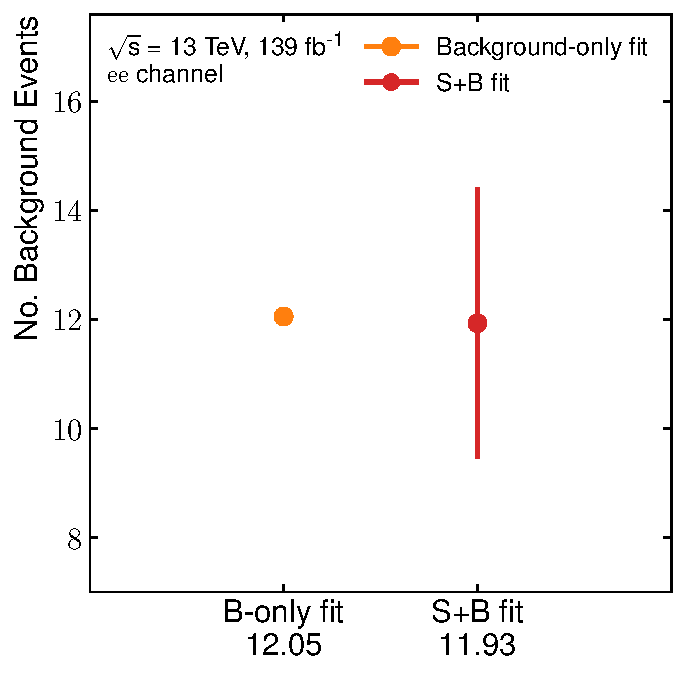
\includegraphics[width=\textwidth]{/Users/Deshan/Documents/PhD/thesis/Thesis/figures/analysis/bkgmodel/nbkg-LL-const-ee.pdf}
        \label{fig:bkgmodel:fitsbplusb1}
    \end{subfigure}
    \begin{subfigure}[b]{0.49\textwidth}
        \centering
        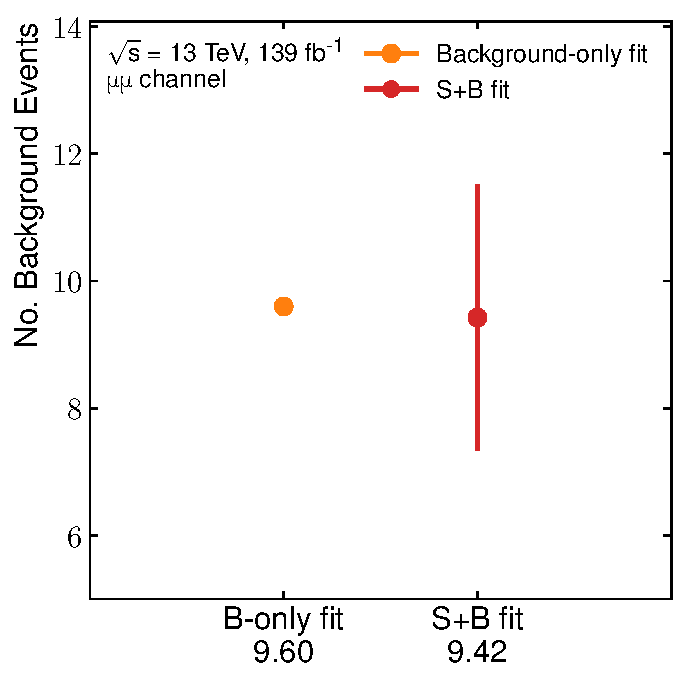
\includegraphics[width=\textwidth]{/Users/Deshan/Documents/PhD/thesis/Thesis/figures/analysis/bkgmodel/nbkg-LL-const-mm.pdf}
        \label{fig:bkgmodel:fitsbplusb2}
    \end{subfigure}
    \begin{subfigure}[b]{0.49\textwidth}
        \centering
        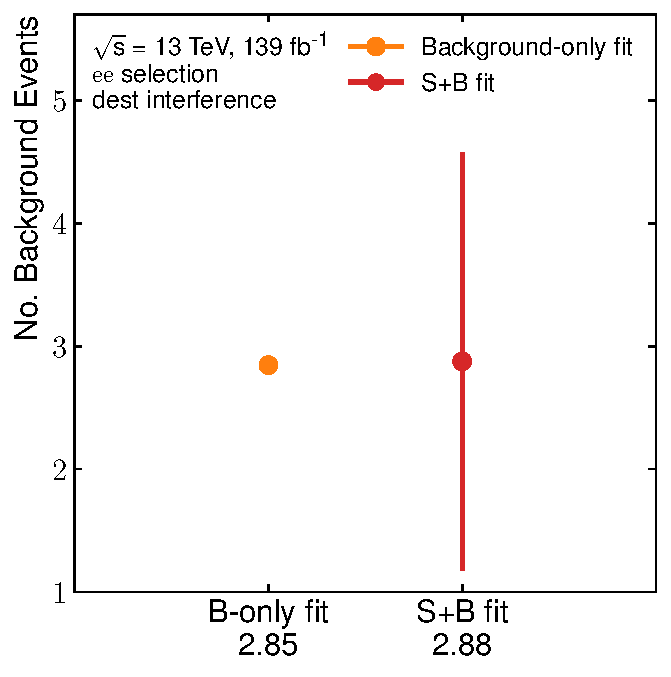
\includegraphics[width=\textwidth]{/Users/Deshan/Documents/PhD/thesis/Thesis/figures/analysis/bkgmodel/nbkg-LL-dest-ee.pdf}
        \label{fig:bkgmodel:fitsbplusb3}
    \end{subfigure}
    \begin{subfigure}[b]{0.49\textwidth}
        \centering
        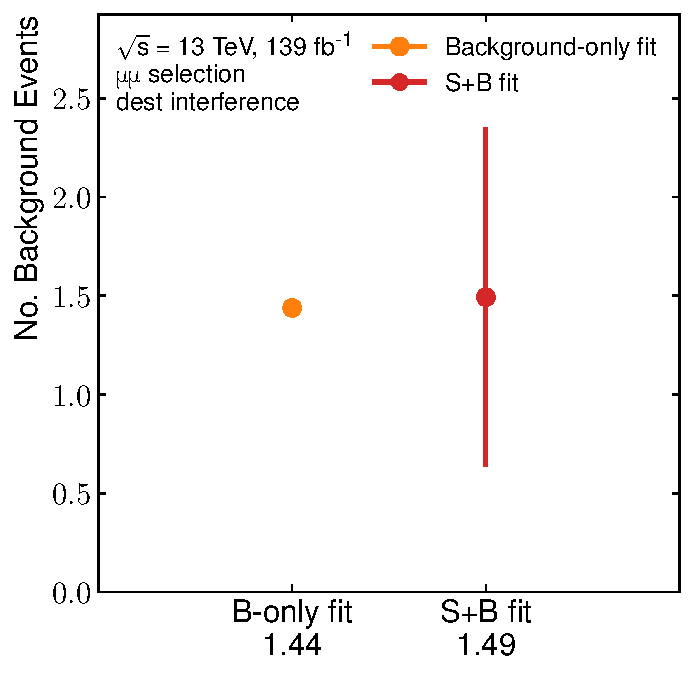
\includegraphics[width=\textwidth]{/Users/Deshan/Documents/PhD/thesis/Thesis/figures/analysis/bkgmodel/nbkg-LL-dest-mm.pdf}
        \label{fig:bkgmodel:fitsbplusb4}
    \end{subfigure}
    \caption[Background estimation comparisons of the signal+background fit and background only fit]{Number of background events in the SR from the background only fit and the signal+background (S+B) fit on MC in the constructive (top) and destructive (bottom) interference SRs for the electron channel (left) and muon channel (right). The uncertainty on the background estimate is shown for background only fit. The number of background events from each fit is shown on the x-axis.}
    \label{fig:bkgmodel:fitsbplusb}
\end{figure}

\begin{figure}[h!]
    \centering
    \begin{subfigure}[b]{0.49\textwidth}
        \centering
        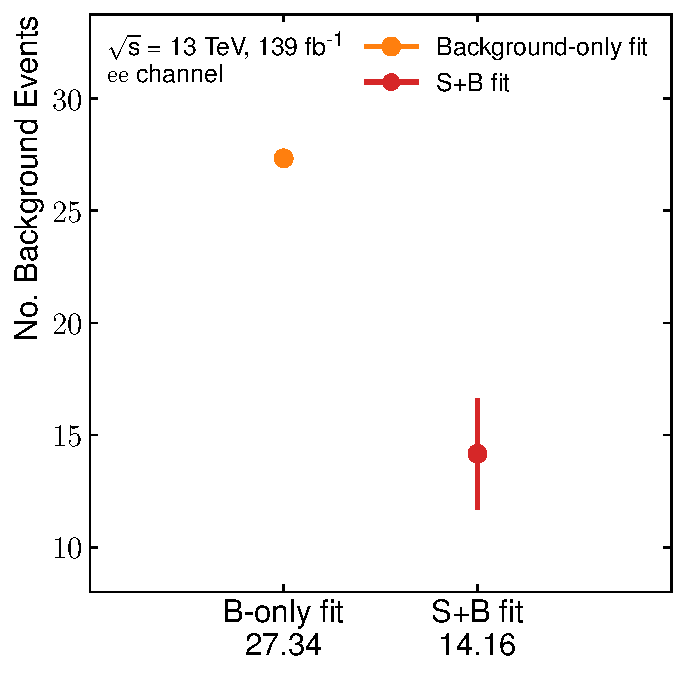
\includegraphics[width=\textwidth]{/Users/Deshan/Documents/PhD/thesis/Thesis/figures/analysis/bkgmodel/nbkg-LL-const-ee-bad.pdf}
        \label{fig:bkgmodel:fitsbplusb1bad}
    \end{subfigure}
    \begin{subfigure}[b]{0.49\textwidth}
        \centering
        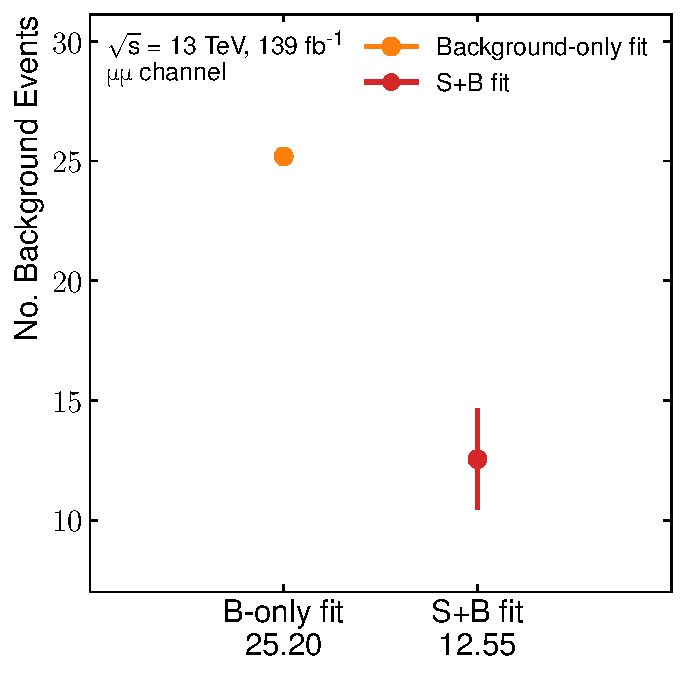
\includegraphics[width=\textwidth]{/Users/Deshan/Documents/PhD/thesis/Thesis/figures/analysis/bkgmodel/nbkg-LL-const-mm-bad.pdf}
        \label{fig:bkgmodel:fitsbplusb2bad}
    \end{subfigure}
    \caption[Background estimation comparisons of the signal+background fit and background only fit in an invalid CR choice.]{Number of background events in the SR from the background-only fit and the signal+background (S+B) fit on data with an injected CI signal with $\Lambda = \SI{18}{\tera\electronvolt}$, for the electron channel (left) and muon channel (right). The uncertainty on the background estimate is shown for background-only fit. The number of background events from each fit is shown on the x-axis.}
    \label{fig:bkgmodel:fitsbplusbbad}
\end{figure}